%\documentclass[12pt]{article}
\documentclass[12pt,landscape]{article}

\usepackage{wrapfig}
%packages
%\usepackage{latexsym}
\usepackage{graphicx}
\usepackage{wrapfig}
\usepackage{color}
\usepackage{amsmath}
\usepackage{dsfont}
\usepackage{placeins}
\usepackage{amssymb}
\usepackage{skull}
\usepackage{enumerate}
\usepackage{soul}
\usepackage{alphalph}
\usepackage{hyperref}
\usepackage{enumerate}
\usepackage{listings}
\usepackage{multicol}
%\usepackage{fancyhdr}

%\fancyhf{} % clear all header and footers
%\renewcommand{\headrulewidth}{0pt} % remove the header rule
%\fancyfoot[LE, LO]{\thepage}


%\usepackage{pstricks,pst-node,pst-tree}

%\usepackage{algpseudocode}
%\usepackage{amsthm}
%\usepackage{hyperref}
%\usepackage{mathrsfs}
%\usepackage{amsfonts}
%\usepackage{bbding}
%\usepackage{listings}
%\usepackage{appendix}
\usepackage[margin=1in]{geometry}
%\geometry{papersize={8.5in,11in},total={6.5in,9in}}
%\usepackage{cancel}
%\usepackage{algorithmic, algorithm}

\definecolor{dkgreen}{rgb}{0,0.6,0}
\definecolor{gray}{rgb}{0.5,0.5,0.5}
\definecolor{mauve}{rgb}{0.58,0,0.82}
\lstset{ %
  language=R,                     % the language of the code
  basicstyle=\footnotesize,       % the size of the fonts that are used for the code
  numbers=left,                   % where to put the line-numbers
  numberstyle=\tiny\color{gray},  % the style that is used for the line-numbers
  stepnumber=1,                   % the step between two line-numbers. If it's 1, each line
                                  % will be numbered
  numbersep=5pt,                  % how far the line-numbers are from the code
  backgroundcolor=\color{white},  % choose the background color. You must add \usepackage{color}
  showspaces=false,               % show spaces adding particular underscores
  showstringspaces=false,         % underline spaces within strings
  showtabs=false,                 % show tabs within strings adding particular underscores
  frame=single,                   % adds a frame around the code
  rulecolor=\color{black},        % if not set, the frame-color may be changed on line-breaks within not-black text (e.g. commens (green here))
  tabsize=2,                      % sets default tabsize to 2 spaces
  captionpos=b,                   % sets the caption-position to bottom
  breaklines=true,                % sets automatic line breaking
  breakatwhitespace=false,        % sets if automatic breaks should only happen at whitespace
  title=\lstname,                 % show the filename of files included with \lstinputlisting;
                                  % also try caption instead of title
  keywordstyle=\color{black},      % keyword style
  commentstyle=\color{dkgreen},   % comment style
  stringstyle=\color{mauve},      % string literal style
  escapeinside={\%*}{*)},         % if you want to add a comment within your code
  morekeywords={*,...}            % if you want to add more keywords to the set
}

\newcommand{\qu}[1]{``#1''}
\newcommand{\spc}[1]{\\ \vspace{#1cm}}

\newcounter{probnum}
\setcounter{probnum}{1}

%create definition to allow local margin changes
\def\changemargin#1#2{\list{}{\rightmargin#2\leftmargin#1}\item[]}
\let\endchangemargin=\endlist 

%allow equations to span multiple pages
\allowdisplaybreaks

%define colors and color typesetting conveniences
\definecolor{gray}{rgb}{0.5,0.5,0.5}
\definecolor{black}{rgb}{0,0,0}
\definecolor{white}{rgb}{1,1,1}
\definecolor{blue}{rgb}{0.5,0.5,1}
\newcommand{\inblue}[1]{\color{blue}#1 \color{black}}
\definecolor{green}{rgb}{0.133,0.545,0.133}
\newcommand{\ingreen}[1]{\color{green}#1 \color{black}}
\definecolor{yellow}{rgb}{1,0.549,0}
\newcommand{\inyellow}[1]{\color{yellow}#1 \color{black}}
\definecolor{red}{rgb}{1,0.133,0.133}
\newcommand{\inred}[1]{\color{red}#1 \color{black}}
\definecolor{purple}{rgb}{0.58,0,0.827}
\newcommand{\inpurple}[1]{\color{purple}#1 \color{black}}
\definecolor{gray}{rgb}{0.5,0.5,0.5}
\newcommand{\ingray}[1]{\color{gray}#1 \color{black}}
\definecolor{backgcode}{rgb}{0.97,0.97,0.8}
\definecolor{Brown}{cmyk}{0,0.81,1,0.60}
\definecolor{OliveGreen}{cmyk}{0.64,0,0.95,0.40}
\definecolor{CadetBlue}{cmyk}{0.62,0.57,0.23,0}

%define new math operators
\DeclareMathOperator*{\argmax}{arg\,max~}
\DeclareMathOperator*{\argmin}{arg\,min~}
\DeclareMathOperator*{\argsup}{arg\,sup~}
\DeclareMathOperator*{\arginf}{arg\,inf~}
\DeclareMathOperator*{\convolution}{\text{\Huge{$\ast$}}}
\newcommand{\infconv}[2]{\convolution^\infty_{#1 = 1} #2}
%true functions

%%%% GENERAL SHORTCUTS

\makeatletter
\newalphalph{\alphmult}[mult]{\@alph}{26}
\renewcommand{\labelenumi}{(\alphmult{\value{enumi}})}
\renewcommand{\theenumi}{\AlphAlph{\value{enumi}}}
\makeatother
%shortcuts for pure typesetting conveniences
\newcommand{\bv}[1]{\boldsymbol{#1}}

%shortcuts for compound constants
\newcommand{\BetaDistrConst}{\dfrac{\Gamma(\alpha + \beta)}{\Gamma(\alpha)\Gamma(\beta)}}
\newcommand{\NormDistrConst}{\dfrac{1}{\sqrt{2\pi\sigma^2}}}

%shortcuts for conventional symbols
\newcommand{\tsq}{\tau^2}
\newcommand{\tsqh}{\hat{\tau}^2}
\newcommand{\sigsq}{\sigma^2}
\newcommand{\sigsqsq}{\parens{\sigma^2}^2}
\newcommand{\sigsqovern}{\dfrac{\sigsq}{n}}
\newcommand{\tausq}{\tau^2}
\newcommand{\tausqalpha}{\tau^2_\alpha}
\newcommand{\tausqbeta}{\tau^2_\beta}
\newcommand{\tausqsigma}{\tau^2_\sigma}
\newcommand{\betasq}{\beta^2}
\newcommand{\sigsqvec}{\bv{\sigma}^2}
\newcommand{\sigsqhat}{\hat{\sigma}^2}
\newcommand{\sigsqhatmlebayes}{\sigsqhat_{\text{Bayes, MLE}}}
\newcommand{\sigsqhatmle}[1]{\sigsqhat_{#1, \text{MLE}}}
\newcommand{\bSigma}{\bv{\Sigma}}
\newcommand{\bSigmainv}{\bSigma^{-1}}
\newcommand{\thetavec}{\bv{\theta}}
\newcommand{\thetahat}{\hat{\theta}}
\newcommand{\thetahatmm}{\hat{\theta}^{\mathrm{MM}}}
\newcommand{\thetahathatmm}{\thetahathat^{\mathrm{MM}}}
\newcommand{\thetahathatmle}{\thetahathat^{\mathrm{MLE}}}
\newcommand{\thetahatmle}{\hat{\theta}^{\mathrm{MLE}}}
\newcommand{\thetavechatmle}{\hat{\thetavec}^{\mathrm{MLE}}}
\newcommand{\muhat}{\hat{\mu}}
\newcommand{\musq}{\mu^2}
\newcommand{\muvec}{\bv{\mu}}
\newcommand{\muhatmle}{\muhat_{\text{MLE}}}
\newcommand{\lambdahat}{\hat{\lambda}}
\newcommand{\lambdahatmle}{\lambdahat_{\text{MLE}}}
\newcommand{\thetahatmap}{\hat{\theta}_{\mathrm{MAP}}}
\newcommand{\thetahatmmae}{\hat{\theta}_{\mathrm{MMAE}}}
\newcommand{\thetahatmmse}{\hat{\theta}_{\mathrm{MMSE}}}
\newcommand{\etavec}{\bv{\eta}}
\newcommand{\alphavec}{\bv{\alpha}}
\newcommand{\minimaxdec}{\delta^*_{\mathrm{mm}}}
\newcommand{\ybar}{\bar{y}}
\newcommand{\xbar}{\bar{x}}
\newcommand{\Xbar}{\bar{X}}
\newcommand{\iid}{~{\buildrel iid \over \sim}~}
\newcommand{\inddist}{~{\buildrel ind \over \sim}~}
\newcommand{\approxdist}{~{\buildrel \bv{\cdot} \over \sim}~}
\newcommand{\equalsindist}{~{\buildrel d \over =}~}
\newcommand{\loglik}[1]{\ell\parens{#1}}
\newcommand{\thetahatkminone}{\thetahat^{(k-1)}}
\newcommand{\thetahatkplusone}{\thetahat^{(k+1)}}
\newcommand{\thetahatk}{\thetahat^{(k)}}
\newcommand{\half}{\frac{1}{2}}
\newcommand{\third}{\frac{1}{3}}
\newcommand{\twothirds}{\frac{2}{3}}
\newcommand{\fourth}{\frac{1}{4}}
\newcommand{\fifth}{\frac{1}{5}}
\newcommand{\sixth}{\frac{1}{6}}

%shortcuts for vector and matrix notation
\newcommand{\A}{\bv{A}}
\newcommand{\At}{\A^T}
\newcommand{\Ainv}{\inverse{\A}}
\newcommand{\B}{\bv{B}}
\renewcommand{\b}{\bv{b}}
\renewcommand{\H}{\bv{H}}
\newcommand{\K}{\bv{K}}
\newcommand{\Kt}{\K^T}
\newcommand{\Kinv}{\inverse{K}}
\newcommand{\Kinvt}{(\Kinv)^T}
\newcommand{\M}{\bv{M}}
\newcommand{\Bt}{\B^T}
\newcommand{\Q}{\bv{Q}}
\newcommand{\Qt}{\Q^T}
\newcommand{\R}{\bv{R}}
\newcommand{\Rt}{\R^T}
\newcommand{\Z}{\bv{Z}}
\newcommand{\X}{\bv{X}}
\newcommand{\Xsub}{\X_{\text{(sub)}}}
\newcommand{\Xsubadj}{\X_{\text{(sub,adj)}}}
\newcommand{\I}{\bv{I}}
\newcommand{\Y}{\bv{Y}}
\newcommand{\sigsqI}{\sigsq\I}
\renewcommand{\P}{\bv{P}}
\newcommand{\Psub}{\P_{\text{(sub)}}}
\newcommand{\Pt}{\P^T}
\newcommand{\Pii}{P_{ii}}
\newcommand{\Pij}{P_{ij}}
\newcommand{\IminP}{(\I-\P)}
\newcommand{\Xt}{\bv{X}^T}
\newcommand{\XtX}{\Xt\X}
\newcommand{\XtXinv}{\parens{\Xt\X}^{-1}}
\newcommand{\XtXinvXt}{\XtXinv\Xt}
\newcommand{\XXtXinvXt}{\X\XtXinvXt}
\newcommand{\x}{\bv{x}}
\newcommand{\w}{\bv{w}}
\newcommand{\q}{\bv{q}}
\newcommand{\zerovec}{\bv{0}}
\newcommand{\onevec}{\bv{1}}
\newcommand{\oneton}{1, \ldots, n}
\newcommand{\yoneton}{y_1, \ldots, y_n}
\newcommand{\yonetonorder}{y_{(1)}, \ldots, y_{(n)}}
\newcommand{\Yoneton}{Y_1, \ldots, Y_n}
\newcommand{\iinoneton}{i \in \braces{\oneton}}
\newcommand{\onetom}{1, \ldots, m}
\newcommand{\jinonetom}{j \in \braces{\onetom}}
\newcommand{\xoneton}{x_1, \ldots, x_n}
\newcommand{\Xoneton}{X_1, \ldots, X_n}
\newcommand{\xt}{\x^T}
\newcommand{\y}{\bv{y}}
\newcommand{\yt}{\y^T}
\renewcommand{\c}{\bv{c}}
\newcommand{\ct}{\c^T}
\newcommand{\tstar}{\bv{t}^*}
\renewcommand{\u}{\bv{u}}
\renewcommand{\v}{\bv{v}}
\renewcommand{\a}{\bv{a}}
\newcommand{\s}{\bv{s}}
\newcommand{\yadj}{\y_{\text{(adj)}}}
\newcommand{\xjadj}{\x_{j\text{(adj)}}}
\newcommand{\xjadjM}{\x_{j \perp M}}
\newcommand{\yhat}{\hat{\y}}
\newcommand{\yhatsub}{\yhat_{\text{(sub)}}}
\newcommand{\yhatstar}{\yhat^*}
\newcommand{\yhatstarnew}{\yhatstar_{\text{new}}}
\newcommand{\z}{\bv{z}}
\newcommand{\zt}{\z^T}
\newcommand{\bb}{\bv{b}}
\newcommand{\bbt}{\bb^T}
\newcommand{\bbeta}{\bv{\beta}}
\newcommand{\beps}{\bv{\epsilon}}
\newcommand{\bepst}{\beps^T}
\newcommand{\e}{\bv{e}}
\newcommand{\Mofy}{\M(\y)}
\newcommand{\KofAlpha}{K(\alpha)}
\newcommand{\ellset}{\mathcal{L}}
\newcommand{\oneminalph}{1-\alpha}
\newcommand{\SSE}{\text{SSE}}
\newcommand{\SSEsub}{\text{SSE}_{\text{(sub)}}}
\newcommand{\MSE}{\text{MSE}}
\newcommand{\RMSE}{\text{RMSE}}
\newcommand{\SSR}{\text{SSR}}
\newcommand{\SST}{\text{SST}}
\newcommand{\JSest}{\delta_{\text{JS}}(\x)}
\newcommand{\Bayesest}{\delta_{\text{Bayes}}(\x)}
\newcommand{\EmpBayesest}{\delta_{\text{EmpBayes}}(\x)}
\newcommand{\BLUPest}{\delta_{\text{BLUP}}}
\newcommand{\MLEest}[1]{\hat{#1}_{\text{MLE}}}

%shortcuts for Linear Algebra stuff (i.e. vectors and matrices)
\newcommand{\twovec}[2]{\bracks{\begin{array}{c} #1 \\ #2 \end{array}}}
\newcommand{\threevec}[3]{\bracks{\begin{array}{c} #1 \\ #2 \\ #3 \end{array}}}
\newcommand{\fivevec}[5]{\bracks{\begin{array}{c} #1 \\ #2 \\ #3 \\ #4 \\ #5 \end{array}}}
\newcommand{\twobytwomat}[4]{\bracks{\begin{array}{cc} #1 & #2 \\ #3 & #4 \end{array}}}
\newcommand{\threebytwomat}[6]{\bracks{\begin{array}{cc} #1 & #2 \\ #3 & #4 \\ #5 & #6 \end{array}}}

%shortcuts for conventional compound symbols
\newcommand{\thetainthetas}{\theta \in \Theta}
\newcommand{\reals}{\mathbb{R}}
\newcommand{\complexes}{\mathbb{C}}
\newcommand{\rationals}{\mathbb{Q}}
\newcommand{\integers}{\mathbb{Z}}
\newcommand{\naturals}{\mathbb{N}}
\newcommand{\forallninN}{~~\forall n \in \naturals}
\newcommand{\forallxinN}[1]{~~\forall #1 \in \reals}
\newcommand{\matrixdims}[2]{\in \reals^{\,#1 \times #2}}
\newcommand{\inRn}[1]{\in \reals^{\,#1}}
\newcommand{\mathimplies}{\quad\Rightarrow\quad}
\newcommand{\mathlogicequiv}{\quad\Leftrightarrow\quad}
\newcommand{\eqncomment}[1]{\quad \text{(#1)}}
\newcommand{\limitn}{\lim_{n \rightarrow \infty}}
\newcommand{\limitN}{\lim_{N \rightarrow \infty}}
\newcommand{\limitd}{\lim_{d \rightarrow \infty}}
\newcommand{\limitt}{\lim_{t \rightarrow \infty}}
\newcommand{\limitsupn}{\limsup_{n \rightarrow \infty}~}
\newcommand{\limitinfn}{\liminf_{n \rightarrow \infty}~}
\newcommand{\limitk}{\lim_{k \rightarrow \infty}}
\newcommand{\limsupn}{\limsup_{n \rightarrow \infty}}
\newcommand{\limsupk}{\limsup_{k \rightarrow \infty}}
\newcommand{\floor}[1]{\left\lfloor #1 \right\rfloor}
\newcommand{\ceil}[1]{\left\lceil #1 \right\rceil}

%shortcuts for environments
\newcommand{\beqn}{\vspace{-0.25cm}\begin{eqnarray*}}
\newcommand{\eeqn}{\end{eqnarray*}}
\newcommand{\bneqn}{\vspace{-0.25cm}\begin{eqnarray}}
\newcommand{\eneqn}{\end{eqnarray}}
\newcommand{\benum}{\begin{itemize}}
\newcommand{\eenum}{\end{itemize}}

%shortcuts for mini environments
\newcommand{\parens}[1]{\left(#1\right)}
\newcommand{\squared}[1]{\parens{#1}^2}
\newcommand{\tothepow}[2]{\parens{#1}^{#2}}
\newcommand{\prob}[1]{\mathbb{P}\parens{#1}}
\newcommand{\littleo}[1]{o\parens{#1}}
\newcommand{\bigo}[1]{O\parens{#1}}
\newcommand{\Lp}[1]{\mathbb{L}^{#1}}
\renewcommand{\arcsin}[1]{\text{arcsin}\parens{#1}}
\newcommand{\prodonen}[2]{\bracks{\prod_{#1=1}^n #2}}
\newcommand{\mysum}[4]{\sum_{#1=#2}^{#3} #4}
\newcommand{\sumonen}[2]{\sum_{#1=1}^n #2}
\newcommand{\infsum}[2]{\sum_{#1=1}^\infty #2}
\newcommand{\infprod}[2]{\prod_{#1=1}^\infty #2}
\newcommand{\infunion}[2]{\bigcup_{#1=1}^\infty #2}
\newcommand{\infinter}[2]{\bigcap_{#1=1}^\infty #2}
\newcommand{\infintegral}[2]{\int^\infty_{-\infty} #2 ~\text{d}#1}
\newcommand{\supthetas}[1]{\sup_{\thetainthetas}\braces{#1}}
\newcommand{\bracks}[1]{\left[#1\right]}
\newcommand{\braces}[1]{\left\{#1\right\}}
\newcommand{\angbraces}[1]{\left<#1\right>}
\newcommand{\set}[1]{\left\{#1\right\}}
\newcommand{\abss}[1]{\left|#1\right|}
\newcommand{\norm}[1]{\left|\left|#1\right|\right|}
\newcommand{\normsq}[1]{\norm{#1}^2}
\newcommand{\inverse}[1]{\parens{#1}^{-1}}
\newcommand{\rowof}[2]{\parens{#1}_{#2\cdot}}

%shortcuts for functionals
\newcommand{\realcomp}[1]{\text{Re}\bracks{#1}}
\newcommand{\imagcomp}[1]{\text{Im}\bracks{#1}}
\newcommand{\range}[1]{\text{range}\bracks{#1}}
\newcommand{\colsp}[1]{\text{colsp}\bracks{#1}}
\newcommand{\rowsp}[1]{\text{rowsp}\bracks{#1}}
\newcommand{\tr}[1]{\text{tr}\bracks{#1}}
\newcommand{\rank}[1]{\text{rank}\bracks{#1}}
\newcommand{\proj}[2]{\text{Proj}_{#1}\bracks{#2}}
\newcommand{\projcolspX}[1]{\text{Proj}_{\colsp{\X}}\bracks{#1}}
\newcommand{\median}[1]{\text{median}\bracks{#1}}
\newcommand{\mean}[1]{\text{mean}\bracks{#1}}
\newcommand{\dime}[1]{\text{dim}\bracks{#1}}
\renewcommand{\det}[1]{\text{det}\bracks{#1}}
\newcommand{\expe}[1]{\mathbb{E}\bracks{#1}}
\newcommand{\expeabs}[1]{\expe{\abss{#1}}}
\newcommand{\expesub}[2]{\mathbb{E}_{#1}\bracks{#2}}
\newcommand{\cexpesub}[3]{\mathbb{E}_{#1}\bracks{#2~|~#3}}
\newcommand{\indic}[1]{\mathds{1}_{#1}}
\newcommand{\var}[1]{\mathbb{V}\text{ar}\bracks{#1}}
\newcommand{\mse}[1]{\mathbb{M}\text{SE}\bracks{#1}}
\newcommand{\sd}[1]{\mathbb{S}\text{D}\bracks{#1}}
\newcommand{\support}[1]{\mathbb{S}\text{upp}\bracks{#1}}
\newcommand{\cov}[2]{\mathbb{C}\text{ov}\bracks{#1, #2}}
\newcommand{\corr}[2]{\mathbb{C}\text{orr}\bracks{#1, #2}}
\newcommand{\se}[1]{\text{SE}\bracks{#1}}
\newcommand{\seest}[1]{\hat{\text{SE}}\bracks{#1}}
\newcommand{\bias}[1]{\mathbb{B}\text{ias}\bracks{#1}}
\newcommand{\partialop}[2]{\dfrac{\partial}{\partial #1}\bracks{#2}}
\newcommand{\secpartialop}[2]{\dfrac{\partial^2}{\partial #1^2}\bracks{#2}}
\newcommand{\mixpartialop}[3]{\dfrac{\partial^2}{\partial #1 \partial #2}\bracks{#3}}

%shortcuts for functions
\renewcommand{\exp}[1]{\mathrm{exp}\parens{#1}}
\renewcommand{\cos}[1]{\text{cos}\parens{#1}}
\renewcommand{\sin}[1]{\text{sin}\parens{#1}}
\newcommand{\sign}[1]{\text{sign}\parens{#1}}
\newcommand{\are}[1]{\mathrm{ARE}\parens{#1}}
\newcommand{\natlog}[1]{\ln\parens{#1}}
\newcommand{\oneover}[1]{\frac{1}{#1}}
\newcommand{\overtwo}[1]{\frac{#1}{2}}
\newcommand{\overn}[1]{\frac{#1}{n}}
\newcommand{\oversqrtn}[1]{\frac{#1}{\sqrt{n}}}
\newcommand{\oneoversqrt}[1]{\oneover{\sqrt{#1}}}
\newcommand{\sqd}[1]{\parens{#1}^2}
\newcommand{\loss}[1]{\ell\parens{\theta, #1}}
\newcommand{\losstwo}[2]{\ell\parens{#1, #2}}
\newcommand{\cf}{\phi(t)}

%English language specific shortcuts
\newcommand{\ie}{\textit{i.e.} }
\newcommand{\AKA}{\textit{AKA} }
\renewcommand{\iff}{\textit{iff}}
\newcommand{\eg}{\textit{e.g.} }
\renewcommand{\st}{\textit{s.t.} }
\newcommand{\wrt}{\textit{w.r.t.} }
\newcommand{\mathst}{~~\text{\st}~~}
\newcommand{\mathand}{~~\text{and}~~}
\newcommand{\ala}{\textit{a la} }
\newcommand{\ppp}{posterior predictive p-value}
\newcommand{\dd}{dataset-to-dataset}

%shortcuts for distribution titles
\newcommand{\logistic}[2]{\mathrm{Logistic}\parens{#1,\,#2}}
\newcommand{\bernoulli}[1]{\mathrm{Bernoulli}\parens{#1}}
\newcommand{\betanot}[2]{\mathrm{Beta}\parens{#1,\,#2}}
\newcommand{\erlang}[2]{\mathrm{Erlang}\parens{#1,\,#2}}
\newcommand{\stdbetanot}{\betanot{\alpha}{\beta}}
\newcommand{\multnormnot}[3]{\mathcal{N}_{#1}\parens{#2,\,#3}}
\newcommand{\normnot}[2]{\mathcal{N}\parens{#1,\,#2}}
\newcommand{\classicnormnot}{\normnot{\mu}{\sigsq}}
\newcommand{\stdnormnot}{\normnot{0}{1}}
\newcommand{\uniform}[2]{\mathrm{U}\parens{#1,\,#2}}
\newcommand{\stduniform}{\uniform{0}{1}}
\newcommand{\exponential}[1]{\mathrm{Exp}\parens{#1}}
\newcommand{\geometric}[1]{\mathrm{Geometric}\parens{#1}}
\newcommand{\gammadist}[2]{\mathrm{Gamma}\parens{#1, #2}}
\newcommand{\negbin}[2]{\mathrm{NegBin}\parens{#1, #2}}
\newcommand{\poisson}[1]{\mathrm{Poisson}\parens{#1}}
\newcommand{\binomial}[2]{\mathrm{Binomial}\parens{#1,\,#2}}
\newcommand{\hypergeom}[3]{\mathrm{Hypergeometric}\parens{#1,\,#2,#3}}
\newcommand{\rayleigh}[1]{\mathrm{Rayleigh}\parens{#1}}
\newcommand{\multinomial}[3]{\mathrm{Multinom}_{#1}\parens{#2,\,#3}}
\newcommand{\gammanot}[2]{\mathrm{Gamma}\parens{#1,\,#2}}
\newcommand{\cauchynot}[2]{\text{Cauchy}\parens{#1,\,#2}}
\newcommand{\invchisqnot}[1]{\text{Inv}\chisq{#1}}
\newcommand{\invscaledchisqnot}[2]{\text{ScaledInv}\ncchisq{#1}{#2}}
\newcommand{\invgammanot}[2]{\text{InvGamma}\parens{#1,\,#2}}
\newcommand{\chisq}[1]{\chi^2_{#1}}
\newcommand{\ncchisq}[2]{\chi^2_{#1}\parens{#2}}
\newcommand{\ncF}[3]{F_{#1,#2}\parens{#3}}

%shortcuts for PDF's of common distributions
\newcommand{\logisticpdf}[3]{\oneover{#3}\dfrac{\exp{-\dfrac{#1 - #2}{#3}}}{\parens{1+\exp{-\dfrac{#1 - #2}{#3}}}^2}}
\newcommand{\betapdf}[3]{\dfrac{\Gamma(#2 + #3)}{\Gamma(#2)\Gamma(#3)}#1^{#2-1} (1-#1)^{#3-1}}
\newcommand{\normpdf}[3]{\frac{1}{\sqrt{2\pi#3}}\exp{-\frac{1}{2#3}(#1 - #2)^2}}
\newcommand{\normpdfvarone}[2]{\dfrac{1}{\sqrt{2\pi}}e^{-\half(#1 - #2)^2}}
\newcommand{\chisqpdf}[2]{\dfrac{1}{2^{#2/2}\Gamma(#2/2)}\; {#1}^{#2/2-1} e^{-#1/2}}
\newcommand{\invchisqpdf}[2]{\dfrac{2^{-\overtwo{#1}}}{\Gamma(#2/2)}\,{#1}^{-\overtwo{#2}-1}  e^{-\oneover{2 #1}}}
\newcommand{\uniformdiscrete}[1]{\mathrm{Uniform}\parens{\braces{#1}}}
\newcommand{\exponentialpdf}[2]{#2\exp{-#2#1}}
\newcommand{\poissonpdf}[2]{\dfrac{e^{-#1} #1^{#2}}{#2!}}
\newcommand{\binomialpdf}[3]{\binom{#2}{#1}#3^{#1}(1-#3)^{#2-#1}}
\newcommand{\rayleighpdf}[2]{\dfrac{#1}{#2^2}\exp{-\dfrac{#1^2}{2 #2^2}}}
\newcommand{\gammapdf}[3]{\dfrac{#3^#2}{\Gamma\parens{#2}}#1^{#2-1}\exp{-#3 #1}}
\newcommand{\cauchypdf}[3]{\oneover{\pi} \dfrac{#3}{\parens{#1-#2}^2 + #3^2}}
\newcommand{\Gammaf}[1]{\Gamma\parens{#1}}

%shortcuts for miscellaneous typesetting conveniences
\newcommand{\notesref}[1]{\marginpar{\color{gray}\tt #1\color{black}}}

%%%% DOMAIN-SPECIFIC SHORTCUTS

%Real analysis related shortcuts
\newcommand{\zeroonecl}{\bracks{0,1}}
\newcommand{\forallepsgrzero}{\forall \epsilon > 0~~}
\newcommand{\lessthaneps}{< \epsilon}
\newcommand{\fraccomp}[1]{\text{frac}\bracks{#1}}

%Bayesian related shortcuts
\newcommand{\yrep}{y^{\text{rep}}}
\newcommand{\yrepisq}{(\yrep_i)^2}
\newcommand{\yrepvec}{\bv{y}^{\text{rep}}}


%Probability shortcuts
\newcommand{\SigField}{\mathcal{F}}
\newcommand{\ProbMap}{\mathcal{P}}
\newcommand{\probtrinity}{\parens{\Omega, \SigField, \ProbMap}}
\newcommand{\convp}{~{\buildrel p \over \rightarrow}~}
\newcommand{\convLp}[1]{~{\buildrel \Lp{#1} \over \rightarrow}~}
\newcommand{\nconvp}{~{\buildrel p \over \nrightarrow}~}
\newcommand{\convae}{~{\buildrel a.e. \over \longrightarrow}~}
\newcommand{\convau}{~{\buildrel a.u. \over \longrightarrow}~}
\newcommand{\nconvau}{~{\buildrel a.u. \over \nrightarrow}~}
\newcommand{\nconvae}{~{\buildrel a.e. \over \nrightarrow}~}
\newcommand{\convd}{~{\buildrel d \over \rightarrow}~}
\newcommand{\nconvd}{~{\buildrel d \over \nrightarrow}~}
\newcommand{\withprob}{~~\text{w.p.}~~}
\newcommand{\io}{~~\text{i.o.}}

\newcommand{\Acl}{\bar{A}}
\newcommand{\ENcl}{\bar{E}_N}
\newcommand{\diam}[1]{\text{diam}\parens{#1}}

\newcommand{\taua}{\tau_a}

\newcommand{\myint}[4]{\int_{#2}^{#3} #4 \,\text{d}#1}
\newcommand{\laplacet}[1]{\mathscr{L}\bracks{#1}}
\newcommand{\laplaceinvt}[1]{\mathscr{L}^{-1}\bracks{#1}}
\renewcommand{\max}[1]{\text{max}\braces{#1}}
\renewcommand{\min}[1]{\text{min}\braces{#1}}

\newcommand{\Vbar}[1]{\bar{V}\parens{#1}}
\newcommand{\expnegrtau}{\exp{-r\tau}}
\newcommand{\cprob}[2]{\prob{#1~|~#2}}
\newcommand{\ck}[2]{k\parens{#1~|~#2}}

%%% problem typesetting
\newcommand{\problem}{\vspace{0.2cm} \noindent {\large{\textsf{Problem \arabic{probnum}~}}} \addtocounter{probnum}{1}}
%\newcommand{\easyproblem}{\ingreen{\noindent \textsf{Problem \arabic{probnum}~}} \addtocounter{probnum}{1}}
%\newcommand{\intermediateproblem}{\noindent \inyellow{\textsf{Problem \arabic{probnum}~}} \addtocounter{probnum}{1}}
%\newcommand{\hardproblem}{\inred{\noindent \textsf{Problem \arabic{probnum}~}} \addtocounter{probnum}{1}}
%\newcommand{\extracreditproblem}{\noindent \inpurple{\textsf{Problem \arabic{probnum}~}} \addtocounter{probnum}{1}}

\newcommand{\easysubproblem}{\ingreen{\item}}
\newcommand{\intermediatesubproblem}{\inyellow{\item}}
\newcommand{\hardsubproblem}{\inred{\item}}
\newcommand{\extracreditsubproblem}{\inpurple{\item}}


\newcounter{numpts}
\setcounter{numpts}{0}


%\newcommand{\subquestionwithpoints}[1]{\addtocounter{numpts}{#1} \item \ingray{[#1 pt]}~~} %  / \arabic{numpts} pts
\newcommand{\subquestionwithpoints}[1]{\addtocounter{numpts}{#1} \item \ingray{[#1 pt / \arabic{numpts} pts]}~~}  
\newcommand{\truefalsesubquestionwithpoints}[1]{\subquestionwithpoints{#1} Record the letter(s) of all the following that are \textbf{true} in general. At least one will be true.}
\newcommand{\multchoicewithpoints}[2]{\subquestionwithpoints{#1} #2}

\newcounter{nummin}
\setcounter{nummin}{0}

\usepackage{accents}
\newlength{\dhatheight}
\newcommand{\doublehat}[1]{%
    \settoheight{\dhatheight}{\ensuremath{\hat{#1}}}%
    \addtolength{\dhatheight}{-0.35ex}%
    \hat{\vphantom{\rule{1pt}{\dhatheight}}%
    \smash{\hat{#1}}}}
\newcommand{\thetahathat}{\doublehat{\theta}}

%\newcommand{\subquestionwithpoints}[1]{\addtocounter{numpts}{#1} \item \ingray{[#1 pt]}~~} %  / \arabic{numpts} pts
\newcommand{\timedsection}[1]{\addtocounter{nummin}{#1}{[#1min] \ingray{(and \arabic{nummin}min will have elapsed)}}}  
%\newcommand{\timedsection}[1]{\addtocounter{nummin}{#1}{[#1 min]}}


\newcommand{\instr}{\small Your answer will consist of a lowercase string (e.g. \texttt{aebgd}) where the order of the letters does not matter. \normalsize}

\title{Math 241 Fall \the\year{} \\ Final Examination}
\author{Professor Adam Kapelner}

\date{Thursday, December 16, \the\year{}}

\begin{document}
\maketitle

%\noindent Full Name \line(1,0){410}

\thispagestyle{empty}

\section*{Code of Academic Integrity}

\footnotesize
Since the college is an academic community, its fundamental purpose is the pursuit of knowledge. Essential to the success of this educational mission is a commitment to the principles of academic integrity. Every member of the college community is responsible for upholding the highest standards of honesty at all times. Students, as members of the community, are also responsible for adhering to the principles and spirit of the following Code of Academic Integrity.

Activities that have the effect or intention of interfering with education, pursuit of knowledge, or fair evaluation of a student's performance are prohibited. Examples of such activities include but are not limited to the following definitions:

\paragraph{Cheating} Using or attempting to use unauthorized assistance, material, or study aids in examinations or other academic work or preventing, or attempting to prevent, another from using authorized assistance, material, or study aids. Example: using an unauthorized cheat sheet in a quiz or exam, altering a graded exam and resubmitting it for a better grade, etc.
\\

\noindent By taking this exam, you acknowledge and agree to uphold this Code of Academic Integrity. \\

%\begin{center}
%\line(1,0){250} ~~~ \line(1,0){100}\\
%~~~~~~~~~~~~~~~~~~~~~signature~~~~~~~~~~~~~~~~~~~~~~~~~~~~~~~~~~~~~~~~~~~~~ date
%\end{center}

\normalsize

\section*{Instructions}
This exam is 110 minutes (variable time per question) and closed-book. You are allowed \textbf{one} page (front and back) of a \qu{cheat sheet}, blank scrap paper and a graphing calculator. Please read the questions carefully. Within each problem, I recommend considering the questions that are easy first and then circling back to evaluate the harder ones. No food is allowed, only drinks. %If the question reads \qu{compute,} this means the solution will be a number otherwise you can leave the answer in \textit{any} widely accepted mathematical notation which could be resolved to an exact or approximate number with the use of a computer. I advise you to skip problems marked \qu{[Extra Credit]} until you have finished the other questions on the exam, then loop back and plug in all the holes. I also advise you to use pencil. The exam is 100 points total plus extra credit. Partial credit will be granted for incomplete answers on most of the questions. \fbox{Box} in your final answers. Good luck!

\pagebreak



%%%%%%%%%%%%%%%%%%
\problem\timedsection{12} The NY state lotto consists of the following game: 6 balls are drawn from a vat of 59 balls by a mechanical ball-picking machine where each ball is labeled 1, 2, \ldots, 59. The 6 numbers on the 6 balls are chosen \emph{uniformly} and \emph{without} replacement and these numbers are called the \qu{lotto draw}. Before the balls are selected, you write down 6 unique numbers from the set $\braces{1, 2, \ldots, 59}$ which is your \qu{lottery ticket}. If your numbers are the same as the 6 numbered balls, you win the lotto \qu{jackpot}. The order of your written numbers doesn't matter. If you have 5 of the 6 numbers correct (and 1 number incorrect), you win the lotto \qu{3rd prize}. If you have 3 numbers written down of the 6 numbered balls (and 3 numbers incorrect), you win the lotto \qu{5th prize}. The order of your written numbers doesn't matter.

\vspace{-0.2cm}\benum\truefalsesubquestionwithpoints{16} 
\begin{enumerate}[(a)]
\item There are 59! ways of arranging all the balls
\item There are 6! / 59! possible lotto draws
\item There are 59! / 6! possible lotto draws
\item The probability of winning the jackpot is 1 in 59!
\item The probability of winning the jackpot is $1 / \binom{59}{6}$
\item The probability of winning a 3rd prize is $53 / \binom{59}{6}$
\item The probability of winning a 3rd prize is $318 / \binom{59}{6}$
\item The probability of winning a 3rd prize is $30 / \binom{59}{6}$
\item The probability of winning a 3rd prize is $6 / \binom{59}{6}$
\item The probability of winning a 3rd prize is $\binom{54}{1} / \binom{59}{6}$
\item The probability of winning a 5th prize is 1/2
\item The probability of winning a 5th prize is $\binom{6}{3}\binom{59}{3} / \binom{59}{6}$
\item The probability of winning a 5th prize is $\binom{6}{3}\binom{53}{3} / \binom{59}{6}$
\item The probability of winning a 5th prize is $\binom{6}{3} / \binom{59}{6}$
\item The count of the numbers you write down which are in the lotto draw can be modeled as $\binomial{6}{1/ \binom{59}{6}}$
\item The count of the numbers you write down which are in the lotto draw can be modeled as $\hypergeom{6}{6}{59}$
\end{enumerate}
\eenum\instr\pagebreak


%%%%%%%%%%%%%%%%%%
\problem\timedsection{5} Winning fifth prize in the lotto has a probability of $p := \binom{6}{3} \binom{53}{3} /  \binom{59}{6} \approx 1\%$. Consider the scenario where you buy one ticket every day and stop buying the day you first win.

\vspace{-0.2cm}\benum\truefalsesubquestionwithpoints{6} 
\begin{enumerate}[(a)]
\item The number of days that go by including the day you stop $T$ in the lotto can be modeled as $T \sim \binomial{n}{p}$ where $n \rightarrow \infty$
\item The number of days that go by including the day you stop $T$ in the lotto can be modeled as $T \sim \geometric{p}$
\item The number of days that go by including the day you stop $T$ in the lotto can be modeled as $T \sim \exponential{np}$ where $n \rightarrow \infty$ 
\item The expected number of days that go by including the day you stop is approximately 100 
\item The expected number of days that go by including the day you stop is approximately 99 
\item The \emph{exact} expected number of days that go by including the day you stop cannot be determined given the information available to you
\end{enumerate}
\eenum\instr\pagebreak


%%%%%%%%%%%%%%%%%%
\problem\timedsection{12} \ingray{Winning fifth prize in the lotto has a probability of $p := \binom{6}{3} \binom{53}{3} /  \binom{59}{6} \approx 1\%$. Consider the scenario where you buy one ticket every day.} Assume $p=1\%$ exactly going forward. The number of days that go by up to and including the day that you \emph{first} win fifth prize $T$ in the lotto can be modeled as $T \sim \geometric{p}$. 

\vspace{-0.2cm}\benum\truefalsesubquestionwithpoints{11} 
\begin{enumerate}[(a)]
\item The probability you win 5th prize on the first day is greater than the probability you win on the 5th prize on the second day
\item The probability you win 5th prize on the first day is equal to the probability you win on the 5th prize on the second day

\item The probability you stop on the first day is greater than the probability you stop on the second day
\item The probability you stop on the first day is equal to the probability you stop on the second day

\item The probability you stop on the first day is equal to the probability you win the 5th prize on the second day

\item The probability you don't win any 5th prizes by day 10 is $1 - .99^{10}$

\item If you know 10 days have passed without winning, the probability you don't win any 5th prizes by day 20 is $1 - .99^{20}$
\item If you know 10 days have passed without winning, the probability you don't win any 5th prizes by day 20 is $1 - .99^{10}$ \\

Each lotto ticket costs \$1 and each winning ticket pays out \$1. So if you lose, you lose \$1 and if you win you get back \$2. 

\item The amount of money you have when you stop is equal to $-T$
\item The amount of money you have when you stop is equal to $1-T$
\item The amount of money you have when you stop is equal to $3-T$
\end{enumerate}
\eenum\instr\pagebreak





%%%%%%%%%%%%%%%%%%
\problem\timedsection{11} \ingray{Winning fifth prize in the lotto has a probability of $p := \binom{6}{3} \binom{53}{3} /  \binom{59}{6} \approx 1\%$. Consider the scenario where you buy one ticket every day.} Assume $p=1\%$ exactly going forward. Now consider we play for exactly 1,000 days. During this time period, we can win multiple times or never win at all.


\vspace{-0.2cm}\benum\truefalsesubquestionwithpoints{17} 
\begin{enumerate}[(a)]
\item The number of 5th prizes you win can be modeled as $\binomial{1000}{0.01}$
\item The number of 5th prizes you win can be modeled as $\hypergeom{1000}{0.01 N}{N}$ where $N$ is very large \\

Each lotto ticket costs \$1 and each winning ticket pays out \$2. So if you lose, you lose \$1 and if you win you get \$2. Denote the payouts by $X_1, X_2, \ldots, X_{1000}$. Let $p_{X_i}(x)$ denote the PMF of $X_i$, $\mu_i$ denote its expectation and $\sigsq_i$ denote its variance. Let $\Xbar$ denote the average of all 1,000 payouts. Let $M_{X_i}(t)$ denote the MGF of $X_i$.

\item $X_1, X_2, \ldots, X_{1000}$ are identically distributed
\item $X_1, X_2, \ldots, X_{1000}$ are independent
\item $\cov{X_1}{X_2} = 0$
\item $\support{X_1} = \braces{-1, 2}$ 
\item $\support{X_1} = \bracks{-1, 2}$ 
\item $p_{X_1}(-1) = 0.99$ 
\item $\mu_1 = -\$0.97$
\item The 5th prize on the lottery is a fair game
\item $\sigsq_1 > 0$
\item $\sigsq_1 = \$0.0891$
\item $\sigma_1 = \$0.0891$
\item $\expe{\Xbar} = \mu_1$
\item $\var{\Xbar} = \sigsq_1$
\item For all realizations, $\displaystyle\frac{x_1 + x_2 + \ldots + x_{1000}}{1000} \approx \mu_1$
\item $M_{X_1}(t) = .01e^{2t} + .99e^{-t}$
\end{enumerate}
\eenum\instr\pagebreak



%%%%%%%%%%%%%%%%%%
\problem\timedsection{10} \ingray{Winning fifth prize in the lotto has a probability of $p := \binom{6}{3} \binom{53}{3} /  \binom{59}{6} \approx 1\%$. Consider the scenario where you buy one ticket every day. Assume $p=1\%$ exactly going forward. Now consider we play for exactly 1,000 days. During this time period, we can win multiple times or never win at all.} Each lotto ticket costs \$1 and each winning ticket pays out \$2. So if you lose, you lose \$1 and if you win you get \$2. Denote the payouts by $X_1, X_2, \ldots, X_{1000}$. These rv's are iid distributed with support $\braces{-1, 2}$, mean $\mu = -\$0.97$ and $\sigsq = 0.0891\$^2$. Let $W = X_1 + X_2 + \ldots + X_{1000}$ denote your \emph{total} winnings over all $1000$ games. Let $Z \sim \stdnormnot$.


\vspace{-0.2cm}\benum\truefalsesubquestionwithpoints{16} 
\begin{enumerate}[(a)]
\item $\expe{W} = -\$0.00097$
\item $\expe{W} = -\$0.97$
\item $\expe{W} = -\$970$
\item $\var{W} = 0.0000891\$^2$
\item $\var{W} = 0.0891\$^2$
\item $\var{W} = 89.1\$^2$

\item $\prob{Z > 0} = \half$
\item $\prob{Z > 1} \approx 16\%$
\item $\prob{Z > -970} \approx 1$
\item $\prob{Z > 970} \approx 0$

\item You have enough information to compute the exact probability of winning, $\prob{W > 0}$
\item $\prob{W > 0} \approx \prob{Z > 0}$ 
\item $\prob{W > 0} \approx \prob{Z > -970}$ 
\item $\prob{W > 0} \approx \prob{Z > -102.7621}$ 
\item $\prob{W > 0} \approx \prob{Z > 102.7621}$ 
\item $\prob{W > 0} \approx 0$
\end{enumerate}
\eenum\instr\pagebreak



%%%%%%%%%%%%%%%%%%
\problem\timedsection{9} \ingray{Winning fifth prize in the lotto has a probability of $p := \binom{6}{3} \binom{53}{3} /  \binom{59}{6} \approx 1\%$. Consider the scenario where you buy one ticket every day. Assume $p=1\%$ exactly going forward. Now consider we play for exactly 1,000 days. During this time period, we can win multiple times or never win at all.} Let $\hat{P}$ denote the sampling distribution for $\hat{p}$, the proportion of 5th prize wins in the $n=1,000$ plays of the lotto.


\vspace{-0.2cm}\benum\truefalsesubquestionwithpoints{13} 
\begin{enumerate}[(a)]
\item $\hat{P} \sim \binomial{1000}{0.01}$
\item $\hat{P} \sim \normnot{10}{9.9}$
\item $\hat{P} \sim \normnot{0.01}{0.0000099}$
\item $\hat{P} \approxdist \normnot{10}{9.9}$
\item $\hat{P} \approxdist \normnot{0.01}{0.0000099}$
\item $\hat{P}$ is approximately normally distributed due to the Binomial Theorem
\item $\hat{P}$ is approximately normally distributed due to the Central Limit Theorem
\item $\hat{P}$ is approximately normally distributed due to the Law of Large Numbers
\item $\hat{P}$ is degenerate-distributed if $n=1$
\item $\hat{P}$ is uniform-distributed if $n=1$
\item $\hat{P}$ is Bernoulli-distributed if $n=1$
\item $\expenoexpand{\hat{P}} = p$
\item $\expenoexpand{\hat{P}} \approx p$ but never exactly equal to $p$ for a finite value of $n$
\end{enumerate}
\eenum\instr\pagebreak



%%%%%%%%%%%%%%%%%%
\problem\timedsection{8} \ingray{Winning fifth prize in the lotto has a probability of $p := \binom{6}{3} \binom{53}{3} /  \binom{59}{6} \approx 1\%$. Consider the scenario where you buy one ticket every day. Assume $p=1\%$ exactly going forward. Now consider we play for exactly 1,000 days. During this time period, we can win multiple times or never win at all. Let $\hat{P}$ denote the sampling distribution for $\hat{p}$, the proportion of 5th prize wins in the $n=1,000$ plays of the lotto. Due to the central limit theorem, $\hat{P} \approxdist \normnot{0.01}{0.00314^2}$.} We are now concerned that the lotto's 5th prize isn't \qu{fair}. This means that we are trying to prove that it is paying out less than what is expected according to probability theory, $p$. Thus we wish to prove that $p < 1\%$.

\vspace{-0.2cm}\benum\truefalsesubquestionwithpoints{9} 
\begin{enumerate}[(a)]

\item This question is an example of statistical inference (which means we try to make inference for an unknown parameter using data)
\item The best, most honest way to prove to others that $p < 1\%$ is to assume $p < 1\%$ is true and then it is believed until it is disproved by data
\item The best, most honest way to prove to others that $p < 1\%$ is to assume $p \geq 1\%$ is true and then let the data disprove $p \geq 1\%$
\item The theory $p < 1\%$ in (c) is called the \qu{alternative hypothesis}
\item The theory $p < 1\%$ in (c) is called the \qu{null hypothesis}

\item The interval $\bracks{0, 1\%}$ is called the set RET, the retainment region for $p$ for some level $\alpha$
\item The interval $\bracks{1\%, 1}$ is called the set RET, the retainment region for $p$ for some level $\alpha$ $RET$
\item The interval $\bracks{0, 1\%}$ is called the set $CI_{p, 1-\alpha}$, the confidence interval for $p$ for some level $\alpha$
\item The interval $\bracks{1\%, 1}$ is called the set $CI_{p, 1-\alpha}$, the confidence interval for $p$ for some level $\alpha$
\end{enumerate}
\eenum\instr\pagebreak


%%%%%%%%%%%%%%%%%%
\problem\timedsection{8} \ingray{Winning fifth prize in the lotto has a probability of $p := \binom{6}{3} \binom{53}{3} /  \binom{59}{6} \approx 1\%$. Consider the scenario where you buy one ticket every day. Assume $p=1\%$ exactly going forward. Now consider we play for exactly 1,000 days. During this time period, we can win multiple times or never win at all. Let $\hat{P}$ denote the sampling distribution for $\hat{p}$, the proportion of 5th prize wins in the $n=1,000$ plays of the lotto. Due to the central limit theorem, $\hat{P} \approxdist \normnot{0.01}{0.00314^2}$. We are now concerned that the lotto's 5th prize isn't \qu{fair}. This means that we are trying to prove that it is paying out less than what is expected according to probability theory, $p$. Thus we wish to prove that $p < 1\%$.} Thus, $H_a: p < 1\%$ and $H_0: p \geq 1\%$. We set $\alpha = 2.5\%$.

\vspace{-0.2cm}\benum\truefalsesubquestionwithpoints{14} 
\begin{enumerate}[(a)]
\item $H_0$ is either retained or rejected
\item If we reject $H_0$, the result is called \qu{statistically significant}.

\item If we reject $H_0$ when $H_0$ was true, this is called a \qu{Type I error}
\item If we reject $H_0$ when $H_0$ was false, this is called a \qu{Type I error}
\item If we retain $H_0$ when $H_0$ was true, this is called a \qu{Type I error}
\item If we retain $H_0$ when $H_0$ was false, this is called a \qu{Type I error}

\item The probability of making a \qu{Type I error} in this test is 2.5\%
\item The probability of making a \qu{Type I error} cannot be computed

\item If $\alpha$ was smaller, the probability of a \qu{Type I error} would increase
\item If $\alpha$ was smaller, the probability of a \qu{Type II error} would increase

\item If the decision is to retain $H_0$, it is possible we made an error
\item If the decision is to reject $H_0$, it is possible we made an error

\item To make a decision about $H_0$, we first construct a set called RET, the retainment region at level $\alpha$.
\item If $\hat{p}$ is an element of the set RET, we reject $H_0$
\end{enumerate}
\eenum\instr\pagebreak


%%%%%%%%%%%%%%%%%%
\problem\timedsection{12} \ingray{Winning fifth prize in the lotto has a probability of $p := \binom{6}{3} \binom{53}{3} /  \binom{59}{6} \approx 1\%$. Consider the scenario where you buy one ticket every day. Assume $p=1\%$ exactly going forward. Now consider we play for exactly 1,000 days. During this time period, we can win multiple times or never win at all. Let $\hat{P}$ denote the sampling distribution for $\hat{p}$, the proportion of 5th prize wins in the $n=1,000$ plays of the lotto. Due to the central limit theorem, $\hat{P} \approxdist \normnot{0.01}{0.00314^2}$. We are now concerned that the lotto's 5th prize isn't \qu{fair}. This means that we are trying to prove that it is paying out less than what is expected according to probability theory, $p$. Thus we wish to prove that $p < 1\%$. Thus, $H_a: p < 1\%$ and $H_0: p \geq 1\%$. We set $\alpha = 2.5\%$.} In the 1,000 days of tickets, we won only 5 times.

\vspace{-0.2cm}\benum\truefalsesubquestionwithpoints{16} 
\begin{enumerate}[(a)]
\item The sample data is the set of 1,000 wins or losses of the 1,000 days of lotto tickets
\item The data were assumed to be sampled iid from a population of infinite size

\item Using the CLT, RET = $\bracks{0, 0.0162}$ rounded to the nearest 3 significant digits
\item Using the CLT, RET = $\bracks{0, 0.0145}$ rounded to the nearest 3 significant digits
\item Using the CLT, RET = $\bracks{0.0162, 1}$ rounded to the nearest 3 significant digits
\item Using the CLT, RET = $\bracks{0.0145, 1}$ rounded to the nearest 3 significant digits

\item Using the CLT, RET = $\bracks{0, 0.00371}$ rounded to the nearest 3 significant digits
\item Using the CLT, RET = $\bracks{0, 0.00554}$ rounded to the nearest 3 significant digits
\item Using the CLT, RET = $\bracks{0.00371, 1}$ rounded to the nearest 3 significant digits
\item Using the CLT, RET = $\bracks{0.00554, 1}$ rounded to the nearest 3 significant digits

\item Using the CLT to compute RET, this test's decision using our data is to reject $H_0$
\item Using the CLT to compute RET, this test's decision using our data is to retain $H_0$

\item If (k) were to be true, a valid conclusion would be \qu{there is sufficient evidence to suggest that NY state is cheating the public out of a fair 5th prize in the lotto}
\item If (l) were to be true, a valid conclusion would be \qu{there is not sufficient evidence to suggest that NY state is cheating the public out of a fair 5th prize in the lotto}

\item Using the CLT, $CI_{p, 95\%} = \bracks{0.000539, 0.00946}$
\item Using the CLT, $CI_{p, 95\%} = \bracks{0.000554, 0.0145}$
\end{enumerate}
\eenum\instr\pagebreak















%%%%%%%%%%%%%%%%%%
\problem\timedsection{11} The time you spend waiting for a bus (measured in minutes) is modeled as $T \sim \exponential{0.2}$, an exponential rv with mean $\mu$ and variance $\sigsq$.

\vspace{-0.2cm}\benum\truefalsesubquestionwithpoints{13} 
\begin{enumerate}[(a)]
\item The PDF of the rv $T$, the bus waiting time is $f(t) = 0.2 e^{-0.2 t}$
\item The PDF of the rv $T$, the bus waiting time is $f(t) = e^{-0.2 t}$
\item $\lim_{t \rightarrow \infty} f(t) = 0$
\item $\lim_{t \rightarrow -\infty} f(t) = 0$
\item $\lim_{t \rightarrow \infty} f(t) = 1$
\item $\lim_{t \rightarrow -\infty} f(t) = 1$
\item The expected waiting time is $\mu$ = 5min
\item There is a 50\% chance you will be waiting for less than 5min
\item You are $e$ times more likely to be waiting 2min than 7min
\item If you were waiting for 5 minutes already, the total expected waiting time is 7.5min
\item The value of $\sigsq$ can be calculated given the information provided to you
\item $\support{T} = \bracks{0, \mu}$
\item $\support{T} = \reals$
\end{enumerate}
\eenum\instr\pagebreak

%%%%%%%%%%%%%%%%%%
\problem\timedsection{12} Let $X \sim U(0, m)$ where $m > 0$. Let $\mu$ denote the expectation of $X$, $\sigsq$ denote the variance of $X$ and $M_X(t) = (e^{mt} - 1) / (mt)$ denote the MGF of $X$.

\vspace{-0.2cm}\benum\truefalsesubquestionwithpoints{14} 
\begin{enumerate}[(a)]
\item $\support{X} = \bracks{0,m}$

\item Let $h(t) := \displaystyle\frac{d}{dt}\bracks{M_X(t)}$. Then $h(0) = m/2$
\item Let $h(t) := \displaystyle\frac{d^2}{dt^2}\bracks{M_X(0)}$. Then $h(0)  = m/2$
\item Let $h(t) := \displaystyle\frac{d}{dt}\bracks{M_X(0)}$. Then $h(0)  = m^2/12$
\item Let $h(t) := \displaystyle\frac{d^2}{dt^2}\bracks{M_X(0)}$. Then $h(0)  = m^2/12$

\item $\expe{X^2} = m^2/12$
\item $\expe{X^2} = m^2/4$
\item $\expe{X^2} = m^2/3$ \\

Let $Y = aX + c$
\item $M_Y(t) = e^{ct}(e^{mt} - 1) / (mt)$
\item $M_Y(t) = e^{ct}(e^{mat} - 1) / (mat)$
\item $M_Y(t) = a(e^{mt} - 1) / (mt) + c$ \\

Let $\Xoneton \iid U(0, m)$ and let $T = X_1 + \ldots + X_n$
\item $M_T(t) =  (e^{mt} - 1)^n / (mt)^n$
\item $M_T(t) =  n(e^{mt} - 1) / (mt)$
\item $M_T(t) =  (e^{mt} - 1) / (mt)$

\end{enumerate}
\eenum\instr\pagebreak




\end{document}





%%% EXPONMENTIAL

%%% MGF












%%%%%%%%%%%%%%%%%%
\vspace{-0.4cm}
\begin{wrapfigure}{R}{2in}
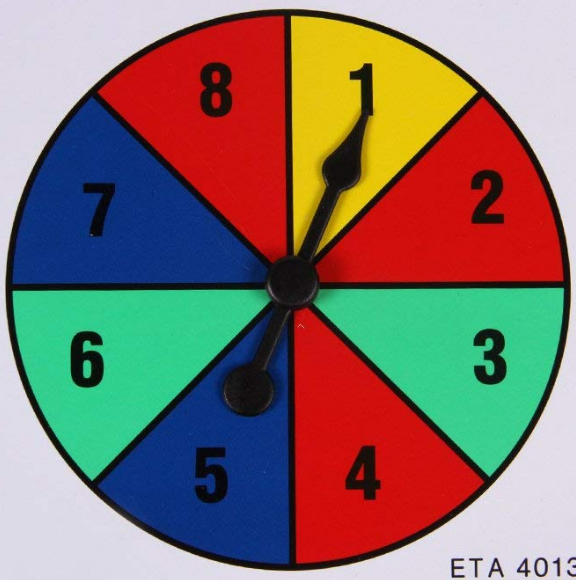
\includegraphics[width=1.5in]{spinner.png}
\end{wrapfigure} \problem\timedsection{12}  Consider a game where someone spins the spinner pictured on the right. The numbers represent payouts in \$. The spinner has four colors: red, blue, green, yellow with payouts 2,4, or 8; 5 or 7; 3 or 6; 1 respectively. Let $X$ be the rv whose realization values are the payouts. Assume the spinner is fair.

\benum\truefalsesubquestionwithpoints{18} 
\begin{enumerate}[(a)]

\vspace{-0.2cm}
\item $X$ is a discrete rv
\item $X$ is a uniform discrete rv
\item $X$ could be a binomial rv where $n = 8$
\item $X$ could be a hypergeometric rv where $N = 8$
\item $\support{X} = \braces{1, 2,..., 8}$
\item $\support{X} = \bracks{1, 8}$
%\item $|\support{X}| = 8$
\item $|\support{X}| = |\naturals|$
\item If we let $\Omega$ = \{Red, blue, green, yellow\} then we can construct a rv $X$ that maps $\omega \in \Omega$ to the support values of $X$.
\item If we let $\Omega = \bracks{0, 2\pi}$ where $\omega$ represents the angle of the spinner from the right horizontal level between states 2 and 3, then we can construct a rv $X$ that maps $\omega \in \Omega$ to the support values of $X$.
\item $\expe{X} = 4$
\item $\expe{X} = 4.5$
\item $\expe{X} = 5$
\item Med$\bracks{X}$ = 4
\item Med$\bracks{X}$ = 4.5
\item Med$\bracks{X}$ = 5
\item Q$\bracks{X, 0.1}$ = 1
\item Q$\bracks{X, 0.1}$ = 2
\item Range$\bracks{X}$ = 8
\end{enumerate}
\eenum\instr\pagebreak

%%%%%%%%%%%%%%%%%%
\begin{wrapfigure}{R}{2in}
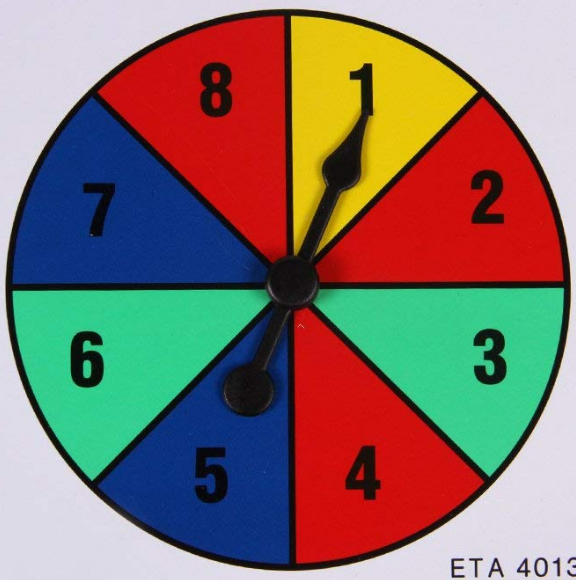
\includegraphics[width=1.5in]{spinner.png}
\end{wrapfigure} \problem\timedsection{8} \ingray{Consider a game where someone spins the spinner pictured on the right. The numbers represent payouts in dollars. The spinner has four colors: red, blue, green, yellow. Red payouts are 2,4, or 8; blue payouts are 5 or 7; green payouts are 3 or 6; yellow only pays out 1. Let $X$ be the rv whose realization values are the payouts. Assume the spinner is fair.} In this rv, $\mu = 4.5$ and $\support{X} = \braces{1, 2,..., 8}$.

\vspace{-0.2cm}\benum\truefalsesubquestionwithpoints{14} 
\begin{enumerate}[(a)]
\item $p(x)$ is monotonically increasing
\item $F(x)$ is monotonically increasing
\item $p(x) < 1$ for all $x \in \support{X}$
\item $F(x) < 1$ for all $x \in \support{X}$
\item $F(4) = 0$
\item $F(4) = 0.5$
\item $F(4) = 1$
\item $p(4) = 0.5$
\item $\sigsq := \var{X} = (1/8) (1^2 + 2^2 + 3^2 + \ldots + 8^2)$
\item $\sigsq := \var{X} = (1/4)(0.5^2 + 1.5^2 + 2.5^2 + 3.5^2)$
\item $\expe{X^2} = 4.5^2$
\item $\sigma := \sd{X} = \expe{X} - 4.5$
\item The unit of the value of the variance of $X$ is dollars
\item The unit of the value of the standard deviation of $X$ is dollars
\end{enumerate}
\eenum\instr\pagebreak

%%%%%%%%%%%%%%%%%%
\begin{wrapfigure}{R}{2in}
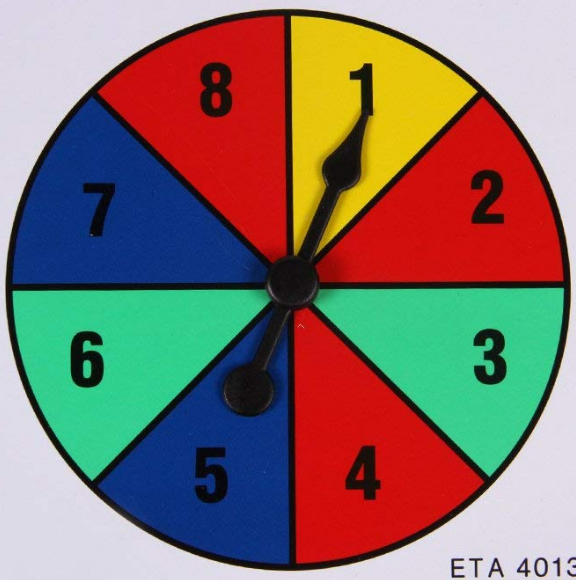
\includegraphics[width=1.3in]{spinner.png}
\end{wrapfigure} \problem\timedsection{10} \ingray{Consider a game where someone spins the spinner pictured on the right. The numbers represent payouts in dollars. The spinner has four colors: red, blue, green, yellow. Red payouts are 2,4, or 8; blue payouts are 5 or 7; green payouts are 3 or 6; yellow only pays out 1. Let $X$ be the rv whose realization values are the payouts. Assume the spinner is fair. In this rv, $\mu = 4.5$ and $\support{X} = \braces{1, 2,..., 8}$.} The variance is $\sigsq := \var{X} = 5.25$ and $\sigma := \sd{X} = 2.29$ rounded to the nearest two digits.

\vspace{-0.2cm}\benum\truefalsesubquestionwithpoints{13} 
\begin{enumerate}[(a)]
\item Another way to define variance (i.e. mean \qu{distance} from the mean) could be $\expe{\abss{X - \mu}}$
\item Another way to define variance (i.e. mean \qu{distance} from the mean) could be $\expe{X - \mu}$
\item Another way to define variance (i.e. mean \qu{distance} from the mean) could be $\expe{(X - \mu)^{100}}$
\item $\expe{X^2} = 5.25 + 4.25^2 = 23.3125$
\item $\expe{X^2} = 5.25 - 4.25^2 = -12.8125$
\item $\expe{X^2} = 5.25^2 - 4.25^2 = 9.5$\\

For the rest of these questions let $Y$ denote the rv for the following game. You play the game $X$ but you have to pay a 20\% of the winnings to the casino, then after the tax is taken, you have to pay \$4 to the casino.

\item $X \equalsindist Y$
\item $X, Y$ are independent rv's
\item $Y$ is a \qu{fair game} for you (the player)
\item $\var{Y} = 0.8\sigsq$
\item $\sd{Y} = 0.8\sigma$
\item The probability of winning money if you play the game $Y$ is 3/8
\item $\var{X + Y}$ would have a non-zero covariance term in its expression
\end{enumerate}
\eenum\instr\pagebreak

%%%%%%%%%%%%%%%%%%
\begin{wrapfigure}{R}{2in}
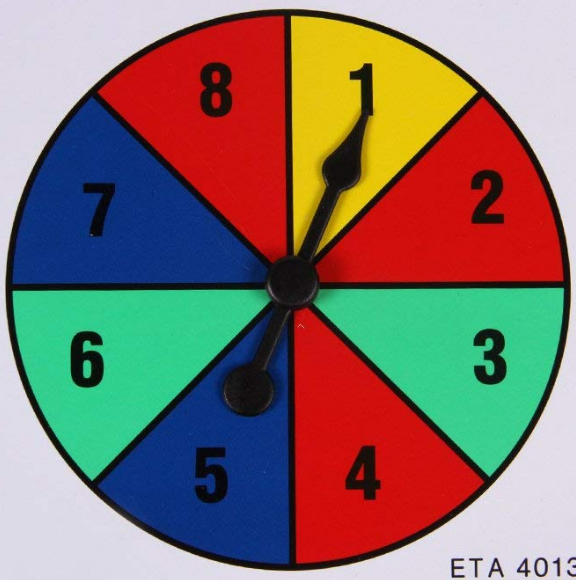
\includegraphics[width=1.5in]{spinner.png}
\end{wrapfigure} \problem\timedsection{9} \ingray{Consider a game where someone spins the spinner pictured on the right. The numbers represent payouts in dollars. The spinner has four colors: red, blue, green, yellow. Red payouts are 2,4, or 8; blue payouts are 5 or 7; green payouts are 3 or 6; yellow only pays out 1. Let $X$ be the rv whose realization values are the payouts. Assume the spinner is fair. In this rv, $\mu = 4.5$ and $\support{X} = \braces{1, 2,..., 8}$. The variance is $\sigsq := \var{X} = 5.25$ and $\sigma := \sd{X} = 2.29$ rounded to the nearest two digits.} Also consider playing this game $n = 1000$ times where the spinner is reset to the same position and you flick it with approximately the same force each time. The payouts for these $n$ games are denoted by rv's $\Xoneton$.

\vspace{-0.2cm}\benum\truefalsesubquestionwithpoints{11} 
\begin{enumerate}[(a)]
\item $\Xoneton \iid$
\item $\Xoneton \inddist$

\item The total winnings after all $n$ games is expected to be $4500$
\item The variance in the total winnings after all $n$ games is 5250
\item The standard deviation in the total winnings after all $n$ games is 72.46 rounded to the nearest two digits.
\item The standard deviation in the total winnings after all $n$ games is 2290

\item The average winnings per game after all $n$ games is expected to be $4.5$
\item The variance in the average winnings per game after all $n$ games is 0.00525
\item The standard deviation in the average winnings per game after all $n$ games is 0.00229 rounded to the nearest 3 digits.
\item The standard deviation in the average winnings per game after all $n$ games is 0.0724 rounded to the nearest 3 digits.
\item As $n$ gets larger, the average winnings per game after all $n$ games approaches a rv centered at $4.5$ with variance shrinking to zero.
\end{enumerate}
\eenum\instr\pagebreak


%%%%%%%%%%%%%%%%%%
\problem\timedsection{9} In the previous game, the probability of winning is $p := 3/8$ and you played $n = 1000$ times. Each game was $\iid$. Let $\Xoneton$ now denote whether each game was won or not (1 = win and 0 = lose). These are different rv's than the previous problem! Let $T$ denote the total number of wins out over the $n$ games.

\vspace{-0.2cm}\benum\truefalsesubquestionwithpoints{17} 
\begin{enumerate}[(a)]
\item $\Xoneton \iid$
\item $X_{17} \sim \bernoulli{3/8}$
\item $X_{17} \sim \bernoulli{5/8}$
\item $T \sim \binomial{n}{p}$
\item $T \sim \hypergeom{n}{np}{n}$ 
\item $T$ is independent of $X_{17}$
\item $\prob{T = 17} = 3/8$
\item $\prob{T = 17} = \binom{1000}{17} (3/8)^{17} (5/8)^{983}$
\item $\prob{X_{17} = 17} = 3/8$
\item $\prob{X_{17} = 17} = (3/8)^{17}$
\item $\prob{X_{17} = 17} = \binom{1000}{17} (3/8)^{17} (5/8)^{983}$
\item $\expe{T} = (3/8)^{17}$
\item $\expe{T} = 1000 \times 3/8$
\item $\var{T} = 1000 \times 3/8 \times 5/8$
\item $\var{T} = \sum_{t=1}^{1000} \binom{1000}{t} (3/8)^{t} (5/8)^{1000 - t}$
\item $\var{T} = \sum_{t=1}^{1000} t \binom{1000}{t} (3/8)^{t} (5/8)^{1000 - t}$
\item If you kept playing this game until you won (i.e. no limit on $n$, the number of games), then the number of games total played would be a memoryless rv.
\end{enumerate}
\eenum\instr\pagebreak


%%%%%%%%%%%%%%%%%%
\problem\timedsection{10} Consider a cup with $N = 8$ coins inside and $K = 3$ coins are marked with a permanent marker. Let $p := 3/8$ denote the proportion of marked coins of the total number of coins. You shake the cup and then reach in and pull out $n = 6$ coins so 6 are in your hand and 2 are left in the cup. Let $X_1, X_2, \ldots, X_6$ denote the rv that models if each of the 6 coins in your hand are marked or unmarked ($X_i = 1$ if marked and $X_i = 0$ if unmarked). Let $T$ denote the number of coins in your hand that are marked with the permanent marker. Thus, $T$ is the sum of $X_1, X_2, \ldots, X_6$.

\vspace{-0.2cm}\benum\truefalsesubquestionwithpoints{16} 
\begin{enumerate}[(a)]
\item $X_1, X_2, \ldots, X_6 \iid$
\item $X_{3} \equalsindist X_6$
\item $X_{3} \sim \bernoulli{p}$
\item $X_{3} \sim \bernoulli{K/N}$
\item $T \sim \binomial{n}{p}$
\item $T \sim \binomial{N}{p}$
\item $T \sim \hypergeom{n}{K}{N}$ 
\item $T \sim \hypergeom{n}{np}{N}$ 
\item $T$ is independent of $X_{3}$
\item $\support{T} = \braces{1, 2, 3, 4, 5, 6, 7, 8}$
\item $\support{T} = \braces{1, 2, 3, 4, 5, 6}$
\item $\support{T} = \braces{1, 2, 3}$
\item $\prob{T = t} = \displaystyle \frac{\binom{3}{t}\binom{5}{6 - t}}{\binom{8}{6}}$
\item $\expe{T} = np$
\item $\expe{T} = n\frac{K}{N}$
\item Given a calculator and enough time, $\var{T}$ can be computed given the information on this page
\end{enumerate}
\eenum\instr\pagebreak

\end{document}


